\begin{surferIntroPage}{世界紀錄曲面}{record_chmutovoktic}{擁有世界紀錄的曲面}
一個不含有任何尖點(這樣點成為奇異點)的曲面被稱為是非奇異的或者光滑的。例如下面兩圖所示的球面或者圓環面。當我們隨機地選擇曲面的時候,非奇異的曲面會很多。
\begin{center}
      \vspace{-0.2cm}
      \begin{tabular}{@{}c@{}c@{}c@{\quad}c@{}c@{}c@{}c@{}}
        \begin{tabular}{@{}c@{}}
          光滑:
        \end{tabular}
        &
        \begin{tabular}{@{}c@{}}
          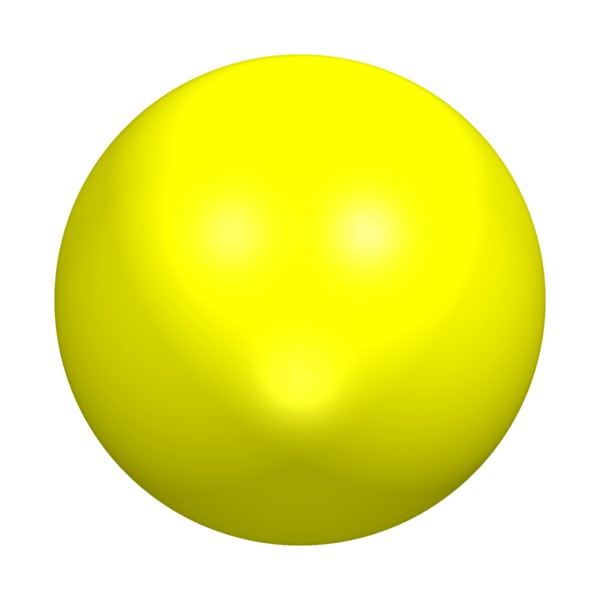
\includegraphics[width=1.1cm]{kugel}
        \end{tabular}
        &
        \begin{tabular}{@{}c@{}}
          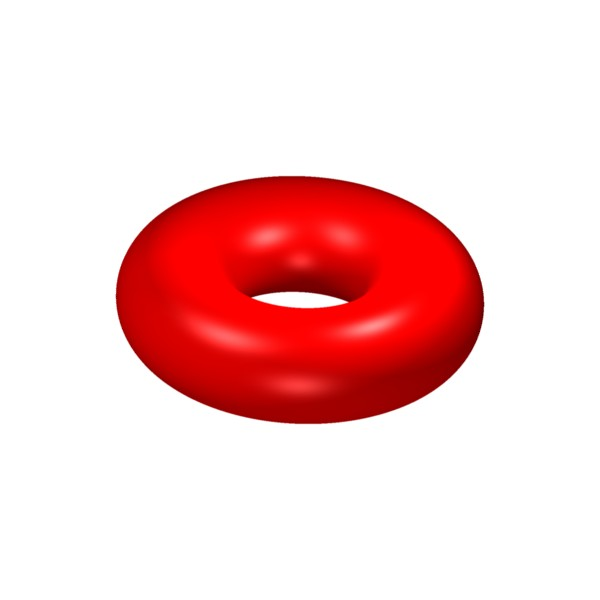
\includegraphics[width=1.1cm]{torus}
        \end{tabular}
        &
        \begin{tabular}{@{}c@{}}
          帶奇點:
        \end{tabular}
        &
        \begin{tabular}{c@{}@{}}
          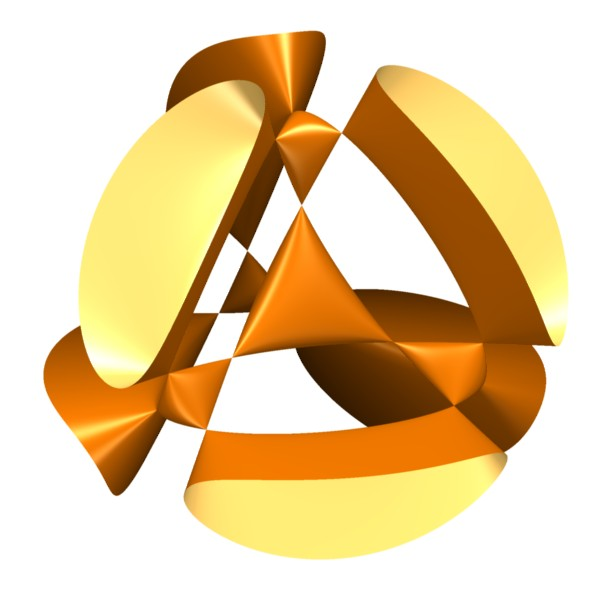
\includegraphics[width=1cm]{kummer}
        \end{tabular}
        &
        \begin{tabular}{c@{}@{}}
          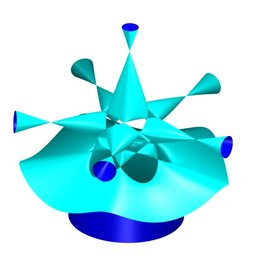
\includegraphics[width=1cm]{togliatti}
        \end{tabular}
        &
        \begin{tabular}{c@{}@{}}
          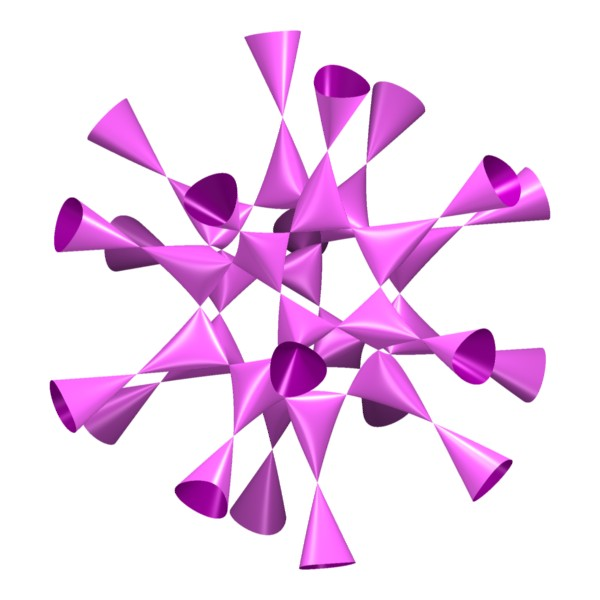
\includegraphics[width=1cm]{barth_sextic}
        \end{tabular}
      \end{tabular}
    \end{center}
    \vspace{-0.2cm}

所以,帶有奇異點的曲面是很特殊的。奇異點是曲面上非常有意思的點。 SURFER 項目中的曲面是由多項式定義的。一個多項式的最高項的次數稱為多項式的次數。
數學家考慮如下問題:一個固定次數的曲面最多會有多少奇異點?我們把這個數目表示為$\mu(d)$。實踐表明,這個數$\mu(d)$非常難以計算。當$d=1,2,3,4$時,19世紀的人們已經知道$\mu(d)$的具體值。但是直到1980年,人們才計算出$\mu(5)$.
$\mu(6)$是1996年被計算出來的。而 $d\ge 7$以及更一般的 $\mu(d)$ 仍然是個未知數。所以關於$\mu(d)$的任何新結果都是非常有重要的。看起來對所有$d$解決這個問題將需要相當長的時間。下面是一些已經知道的結果:
   \begin{center}
      \begin{tabular}{r|cccccccc|c}
        $d$ & $1$ & $2$ & $3$ & $4$ & $5$ & $6$ & $7$ & $8$ & $d$\\
        \hline
        \hline
        \rule{0pt}{1.2em}$\mu(d)\ge$ & $0$ & $1$ & $4$ & $16$ & $31$ & $65$ &
        $99$ & $168$ &
        $\approx \frac{5}{12}d^3$\\[0.3em]
        \hline
        \rule{0pt}{1.2em}$\mu(d)\le$ & $0$ & $1$ & $4$ & $16$ & $31$ & $65$ &
        $104$ & $174$ & $\approx \frac{4}{9}d^3$
      \end{tabular}
    \end{center}
\end{surferIntroPage}
